\documentclass[a4paper,11pt]{article}

\usepackage[margin=2cm]{geometry}
\usepackage[english]{babel}
\usepackage[utf8]{inputenc}
\usepackage[T1]{fontenc}
\usepackage{lmodern}

\usepackage{float}
\usepackage{graphicx}
\usepackage{enumerate}
\usepackage{booktabs}
\usepackage{xcolor}
\usepackage{hyperref}
\hypersetup{
    colorlinks,
    linkcolor={red!50!black},
    citecolor={blue!50!black},
    urlcolor={blue!80!black}
}

\title{Embedded Systems project report}
\author{}
\date{\today}

\begin{document}

\maketitle
\tableofcontents

\section{Project Data}

\begin{table}[H]
  \centering
  \begin{tabular}{ll}
    \toprule
    Supervisors   & Davide Galli, Davide Zoni \\
    Participants  & Alexandru Gabriel Bradatan - 10658858 \\
    Tags          & Complex \\
    \bottomrule
  \end{tabular}
\end{table}

\section{Project Description}

CVA6 is a 6-stage in-order and single issue processor core which implements the
RISC-V instruction set with the I, M, A and C extensions. CVA6 can be configured
as a 32- or 64-bit core (RV32 or RV64), called CV32A6 or CV64A6. It also implements three
privilege levels M, S, U to fully support a Unix-like operating system, like Linux.
It is fully open source (\href{https://github.com/openhwgroup/cva6}{repository})
and written in SystemVerilog.

This project has two main goals:

\begin{enumerate}
  \item Instantiate a CVA6 core
  \item Boot a Linux image on a simulated CVA6 testbench and execute some programs
\end{enumerate}

We are going to work on the latest release of the CVA6 core (5.1.0) and use
Vivado 2023.2 as an IDE and synthesis tool, while a customized version of Verilator
as a simulator.

All artifacts of this project are available in \href{https://github.com/alexbradd/embedded-systems-project-2024}{this repository}
together with instructions and scripts for cloning, opening the project in Vivado and
compiling the necessary software for starting a simulation.

\subsection{CVA6 Instance}

The FPGA used for synthesis is and Artix-7, specifically
\texttt{xc7a35tcsg324-1}. This part has been chosen mainly because it is the one
found on the entry level Arty A7-35T board and it is just enough for what we
need.

To instantiate a CVA6 core, we must create a Verilog module describing a minimal
SoC composed of the CVA6 core and some essential peripherals, which are the
Core-Level interrupt controller (for the timer interrupt) and the DRAM, all
connected together by an AXI crossbar. The resulting module will receive as inputs
the clock from the board's oscillator, the reset signal and other auxiliary signals
for interfacing with the onboard memory.

Our board provides one 100MHz oscillator. This clock will feed directly into
Xilinx's DDR3 memory IP running at 325 MHz. This frequency has so that it takes an input of
100MHz. The MIG IP outputs a \texttt{ui\_clk} clock with frequency $325 / 4 = 81.25$
MHz. This signal, reassigned to \texttt{dram\_clk} for naming clarity, will be
rescaled by the Clock Wizard Xilinx IP into 2 clocks:

\begin{enumerate}
  \item A 200 MHz reference clock used by the DRAM
  \item A 50 MHz clock used by the CPU and its peripherals
\end{enumerate}

Since the memory and the AXI bus it needs to interface are in two different
clock domains, we also need to correctly cross clock domains. This is handled by
the AXI Clock Converter Xilinx IP. A diagram of the module's clock generation is
provided in Figure~\ref{clock-diag}.

\begin{figure}
  \centering
  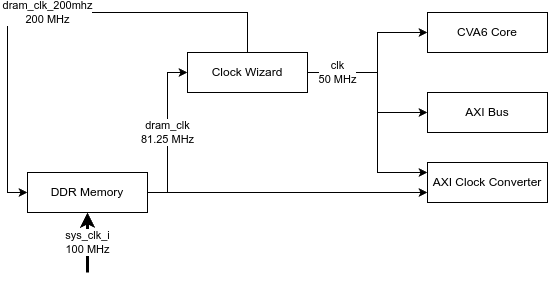
\includegraphics[width=\textwidth]{./img/clocking_diagram.png}
  \caption{Diagram of the clock generation}%
  \label{clock-diag}
\end{figure}

The configuration of the CVA6 core used for this implementation is the
\texttt{CV32A6\_IMA\_SV32\_FPGA} config.

This design is implemented in the \texttt{synth\_harness} module. The synthesis
succeeds and results in the resource usage outline in Table~\ref{synth-util}.

\begin{table}[H]
  \centering
  \begin{tabular}{lrrr}
    \toprule
    Resource & Utilization & Available & Utilization \% \\\midrule
    LUT      & 16421       & 20800     & 78.95 \% \\
    FF       & 12096       & 41600     & 29.08 \% \\
    BRAM     & 16.50       & 50        & 33.00 \% \\
    DSP      & 4           & 90        &  4.44 \% \\
    IO       & 50          & 210       & 23.81 \% \\
    MMCM     & 2           & 5         & 40.00 \% \\
    PLL      & 1           & 5         & 20.00 \% \\
    \bottomrule
  \end{tabular}
  \caption{Post-synthesis utilization report}%
  \label{synth-util}
\end{table}

\subsection{CVA6 Simulation}

As mentioned previously, to have maximum compatibility with both the upstream
Verilog code and any upstream scripts that may be needed, we have decided to use
Verilog compiled with the in-tree patches. The same logic will be applied to any
other auxiliary tools required for simulation.

The choice of not using Vivado as the simulator
has been made due to it not being able to correctly parse some otherwise valid
Verilog code (specifically
\href{https://github.com/openhwgroup/cva6/blob/db088159ebca1480b3c5f083f5ac4268ea6749b6/vendor/pulp-platform/common_cells/include/common_cells/registers.svh#L47}{this} and
\href{https://github.com/openhwgroup/cva6/blob/db088159ebca1480b3c5f083f5ac4268ea6749b6/vendor/pulp-platform/common_cells/include/common_cells/registers.svh#L125}{this} lines).

The simulation testbench used is the one provided by upstream. It comprises of a
\texttt{CV64A6\_IMAFDC\_SV39} core, a JTAG module, a behavioural SRAM for the
image and a behavioural UART.

Compilation of the tools with the host compiler, compilation of the cross compiler
and cross compilation of the Linux image are handled by scripts provided by the
main repo and an \href{https://github.com/openhwgroup/cva6-sdk}{SDK} repo.

Invocation of the build scripts with the correct parameters has been automated by us
with a Makefile. To compile all tools and images needed for simulation, one can execute
simply execute \texttt{make tools}.

Simulation is started by invoking an upstream provided Python script with the
ELF image to run and desired board configuration. As with compilation, correct
invocation has been implemented as a Make target: one can simply execute
\texttt{make sim} to start a simulation of the core running the built Linux
image.

To connect to the simulated core, one can use OpenOCD with JTAG Remote BitBang.
A simple OpenOCD configuration to connect to the core has been provided in the
project repo.

\section{Project Outcomes}

\subsection{Concrete Outcomes}

The project created a Verilog module that correctly instantiates a configuration
of the CVA6 core and synthesizes correctly.

The project also built upon the tools provided by the upstream developers to
enable us to easily build a RISCV Linux image and start a simulation of a CVA6
core running said image using Verilator.

\subsection{Problems encountered}

Unfortunately, we were not able to get a shell prompt through the simulated UART
and execute programs. Adding to the problems is the fact that we could not find
documentation for simulating a full OS image. This left us with only
trial and error and reverse engineering scripts, both of which are very time
consuming.

To connect to the core, we tried using OpenOCD with the simple configuration
contained in the project repo. While the simulation was running fine on its own,
once we tried to connect to it the connection would be established, but the
whole thing would crash after a some time (usually a around a couple of
minutes). The OpenOCD output is the following:

\begin{verbatim}
Open On-Chip Debugger 0.12.0
Licensed under GNU GPL v2
For bug reports, read
    http://openocd.org/doc/doxygen/bugs.html
DEPRECATED! use 'adapter speed' not 'adapter_khz'
Info : only one transport option; autoselect 'jtag'
Warn : `riscv set_prefer_sba` is deprecated. Please use
    `riscv set_mem_access` instead.
Info : Initializing remote_bitbang driver
Info : Connecting to localhost:9824
Info : remote_bitbang driver initialized
Info : This adapter doesn't support configurable speed
Info : JTAG tap: riscv.cpu tap/device found:
    0x00000001 (mfg: 0x000 (<invalid>), part: 0x0000, ver: 0x0)
Info : datacount=2 progbufsize=8
Error: unable to halt hart 0
Error:   dmcontrol=0x80000001
Error:   dmstatus =0x00000c82
Error: Fatal: Hart 0 failed to halt during examine()
Warn : target riscv.cpu examination failed
Info : starting gdb server for riscv.cpu on 3333
Info : Listening on port 3333 for gdb connections
Error: Target not examined yet
Info : remote_bitbang interface quit
\end{verbatim}

We think that this may be caused by an incorrect configuration of OpenOCD or of
the testbench. We are very sure that the problem was neither the fact that Linux
is unsupported or that the image is built incorrectly since for the former
there are some (now broken) scripts that can boot a Linux image, and for the
latter we used the official SDK with the default options and without any
modification.

Another possibility may be that OpenOCD is not supported and the UART would use
the same TTY as the simulation script for communication. This seems not to be
the case because even after waiting for several minutes, the scripts output
doesn't display anything other some debug information related to invocation
arguments. To be sure, we would need to reverse the whole simulation script.

Lastly we would like to add that we are sure that the simulation is working since
something is being executed. We can see from the utilization of our physical CPUs
the simulation is consuming CPU time meaning that either the CPU is doing
something.

\end{document}
